\documentclass{article}
\usepackage{listings}
\usepackage{graphicx}
\usepackage{fancyhdr}
\usepackage{xcolor}
\usepackage{subcaption}
\usepackage{biblatex}

\definecolor{codegreen}{rgb}{0,0.6,0}
\definecolor{codegray}{rgb}{0.5,0.5,0.5}
\definecolor{codepurple}{rgb}{0.58,0,0.82}
\definecolor{backcolour}{rgb}{0.95,0.95,0.92}

% \lstdefinestyle{mystyle}{
%   backgroundcolor=\color{backcolour}, commentstyle=\color{codegreen},
%   keywordstyle=\color{magenta},
%   numberstyle=\tiny\color{codegray},
%   stringstyle=\color{codepurple},
%   basicstyle=\ttfamily\footnotesize,
%   breakatwhitespace=false,         
%   breaklines=true,                 
%   captionpos=b,                    
%   keepspaces=true,                 
%   numbers=left,                    
%   numbersep=5pt,                  
%   showspaces=false,                
%   showstringspaces=false,
%   showtabs=false,                  
%   tabsize=2
% }

\bibliography{testcases.bib}

% \lstset{style=mystyle}
\lstset{basicstyle=\ttfamily,
  showstringspaces=false,
  commentstyle=\color{red},
  keywordstyle=\color{blue}
}



\title{CS108 Bash Grader Testcases and Explanation}
\author{Aditya Neeraje : 23B0940}
\date{April 28, 2024}
\graphicspath{{./Images/}}

\begin{document}
    \maketitle
    \clearpage
    \section{Initialize}
    Running the following command initializes 4 csv files with random data and combines some of this data into main.csv.
    \begin{lstlisting}[language=bash]
        python3 initialize.py
    \end{lstlisting}
    \begin{figure}[htbp]
        \centering
        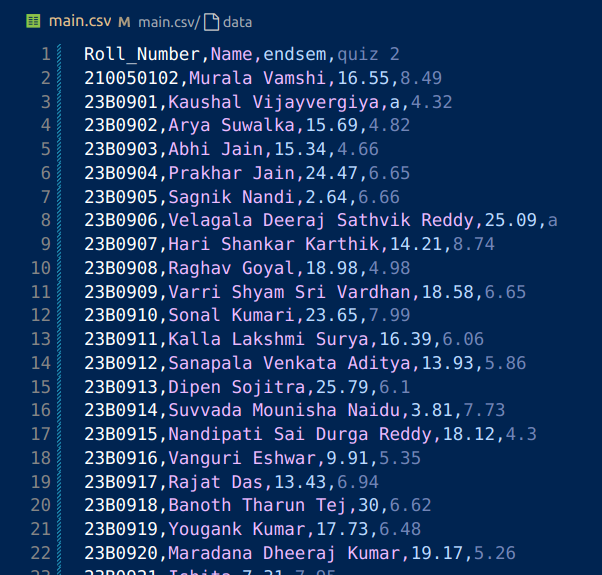
\includegraphics[width=0.4\textwidth]{Initialize}
        \caption{main.csv after Initializing}
        \label{fig:initialize}
    \end{figure}

    \section{Combine}
    Running the following command combines the data from 4 csv files into main.csv.
    \begin{lstlisting}[language=bash]
        bash submission.sh combine
    \end{lstlisting}
    \begin{figure}[htbp]
        \centering
        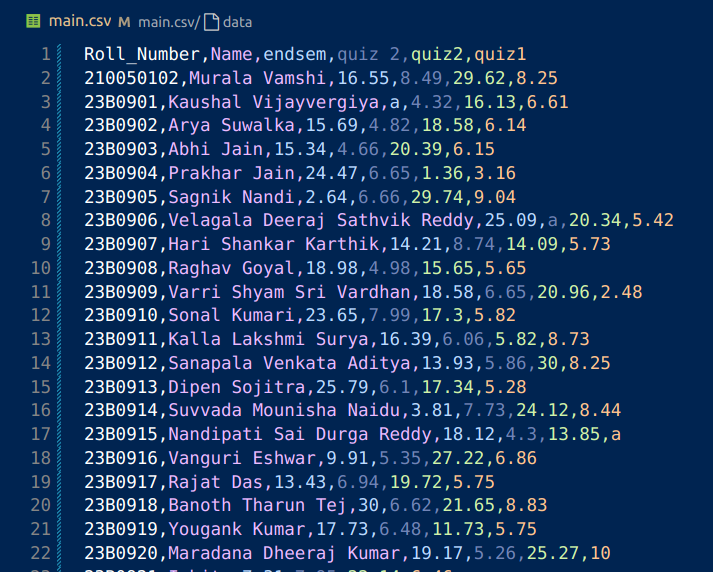
\includegraphics[width=0.4\textwidth]{Combine_all}
        \caption{main.csv after combining all 4}
        \label{fig:combine_all}
    \end{figure}

    You can specify files to drop by passing them as arguments to the script.
    \begin{lstlisting}[language=bash]
        bash submission.sh combine --drop quiz1.csv "quiz 2.csv"
        bash submission.sh combine -d quiz1.csv "quiz 2.csv"
    \end{lstlisting}
    \begin{figure}[htbp]
        \centering
        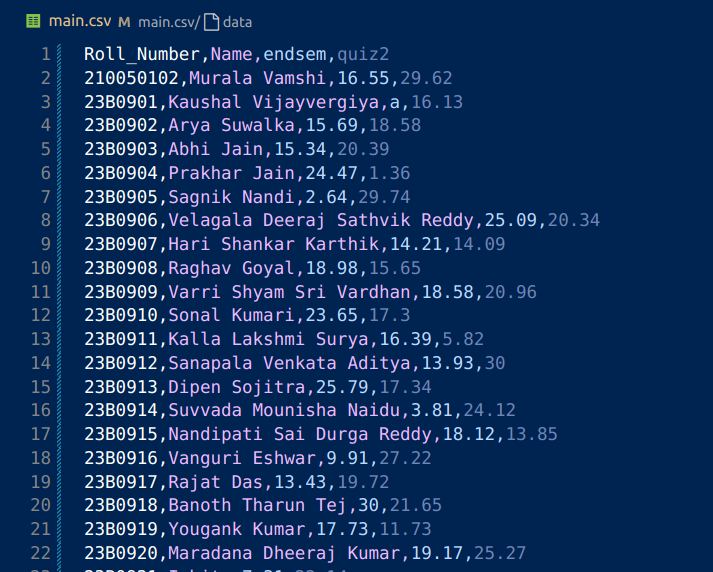
\includegraphics[width=0.4\textwidth]{Drop_two_quizzes}
        \caption{main.csv after dropping quiz1.csv and quiz 2.csv}
        \label{fig:combine_drop}
    \end{figure}

    You can selectively combine back certain quizzes alone by passing them as arguments before any other flag.
    \begin{lstlisting}[language=bash]
        bash submission.sh combine quiz1.csv
    \end{lstlisting}
    \begin{figure}[htbp]
        \centering
        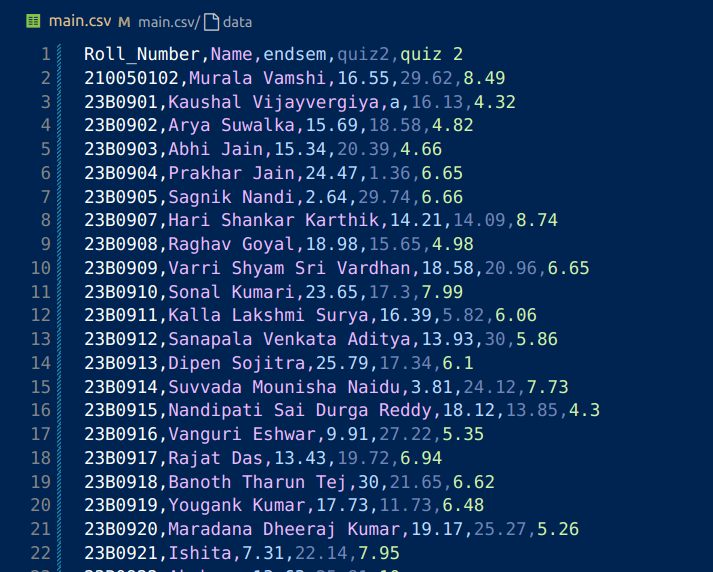
\includegraphics[width=0.4\textwidth]{Combine_quiz_2.png}
        \caption{main.csv after combining quiz 2.csv}
        \label{fig:combine_quiz1}
    \end{figure}

    Generally, combine does not recheck or recombine quizzes which already have a column assigned to them in main.csv, and whose first 3 lines of data are valid marks. Use the --force flag to combine them.
    \begin{lstlisting}
        bash submission.sh combine quiz1.csv quiz2.csv "quiz 2.csv" --force
    \end{lstlisting}
    \begin{figure}[htbp]
        \centering
        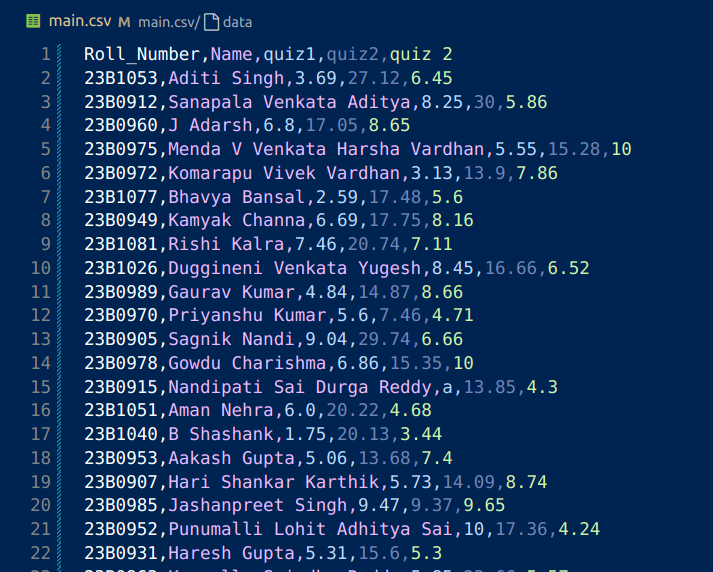
\includegraphics[width=0.4\textwidth]{Force_flag}
        \caption{main.csv after combining all but endsem with force}
        \label{fig:combine_quiz1_force}
    \end{figure}
    Note here that endsem.csv is actually lost from main, since both the force\_flag and the only\_flag are true and endsem.csv is not amongst the list of quizzes to only add to main.
        
    combine also works as intended if main.csv is not present in the \texttt{WORKING\_DIRECTORY}, creating main.csv. All flags work similarly as to the normal case. The user might notice non-fatal errors being registered due to head trying to read the non-existent main.csv file. This is expected behavior.
    Similarly, combine works as intended even if main.csv is empty (such as by running \texttt{echo "" > main.csv}).

    \section{Rescale}
    Rescale can accept arguments as a list of weights, or as a custom series of quiz\_names and weights. The first way can be achieved through the \texttt{-w}/\texttt{--weights-only} flag, or by passing no flag.
    \begin{lstlisting}
        bash submission.sh rescale -w 1 2 1 1
    \end{lstlisting}
    \begin{figure}[htbp]
        \centering
        \begin{subfigure}[b]{0.45\textwidth}
            \centering
            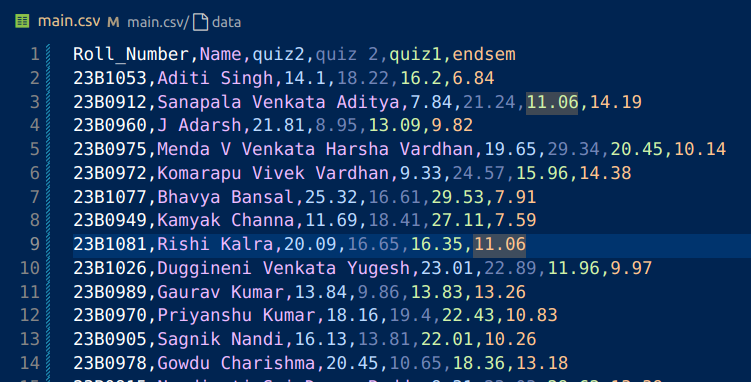
\includegraphics[width=\textwidth]{Before_Rescale}
            \caption{Before Rescale}
            \label{fig:bef_res}
        \end{subfigure}
        \hfill
        \begin{subfigure}[b]{0.45\textwidth}
            \centering
            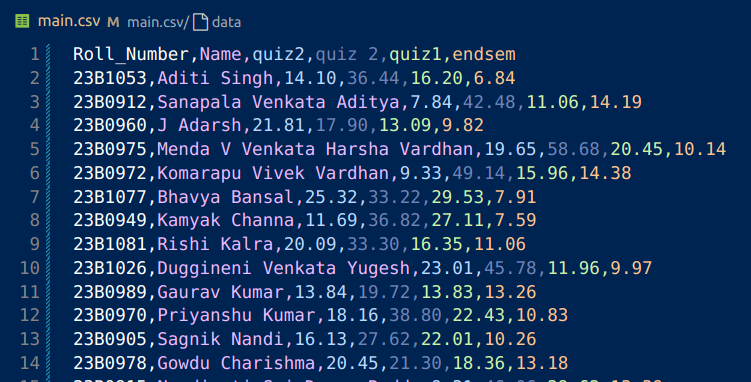
\includegraphics[width=\textwidth]{After Rescale.png}
            \caption{After Rescale}
            \label{fig:aft_res}
        \end{subfigure}
        \caption{Rescale with weights 1 2 1 1}
        \label{fig:bef_and_aft_rescale}
    \end{figure}

    If you do not pass as many weights as there are quizzes, the script will prompt for more weights in order of the quizzes' appearance in main.csv.
    \begin{figure}[htbp]
        \centering
        \includegraphics[width=0.8\textwidth]{Prompt for weights}
        \caption{Prompting user for weights}
        \label{fig:prompt_weights}
    \end{figure}

    It is worth noting that if the user enters invalid entries, the prompts will continue until a valid weight is given.\\
    As is the default with the \texttt{bc} command on bash, non-numeric values such as \lq\lq a\rq\rq\ or \lq\lq hello\rq\rq\ get translated to 0, whereas invalid entries include entries such as \lq\lq 1.2.3\rq\rq\ or \lq\lq 1/0\rq\rq\ or \lq\lq 1/\rq\rq, etc.\\
    The fact that rescale runs bc in the background on the weights inputted means that the weights can be in the form of expressions such as 2\^4, 1/3, etc. To pass longer expressions with spaces (such as 1 + 1 + 1), either enclose the expressions in brackets or pass them using -c flag, which uses the \texttt{read} command instead of considering each word a new argument. \\
    \begin{figure}[htbp]
        \centering
        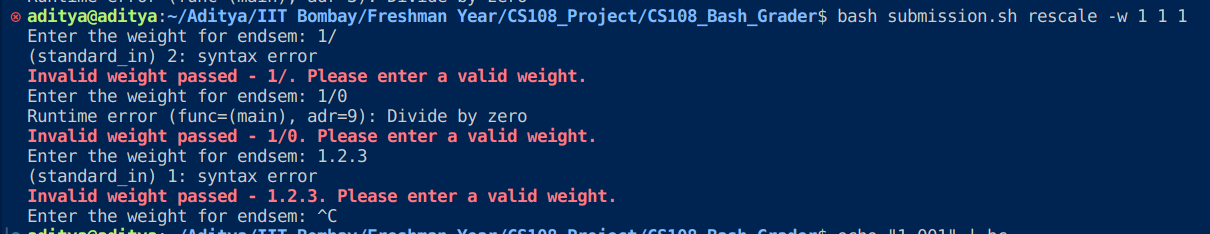
\includegraphics[width=0.8\textwidth]{Prompting_for_Correct_Weights}
        \caption{The script prompts the user until correct data is entered.}
        \label{fig:rescale_expr}
    \end{figure}

    The \texttt{-c}/\texttt{--custom} flag allows you to pass a custom series of quiz names and weights. The script will assume the weights of the quizzes not mentioned in the custom series are 1.\\
    Quiz names are to be passed to the prompt as basenames only, without .csv extensions. If the same quiz name is passed twice, only the second corresponding weight is considered.\\
    Ctrl+D is used to signal the end of the input.\\

    \section{Upload}
    Upload is fairly simple. It checks for the existence of the given file, checks for validity of the data in the given file (i.e the header format and that all quiz marks must be numeric or "a"). It prompts for user permission if the upload would overwrite a file already in the \texttt{WORKING\_DIRECTORY}, unless the \texttt{--force} flag is passed.\\
    By default, Upload calls Combine after uploading, as this is the expected usage of my script.\\
    For example, if ../quizzz.csv is the file to be uploaded, the following command will upload the file and combine it with main.csv.
    \begin{lstlisting}
        bash submission.sh upload ../quizzz.csv
    \end{lstlisting}
    \begin{figure}[htbp]
        \centering
        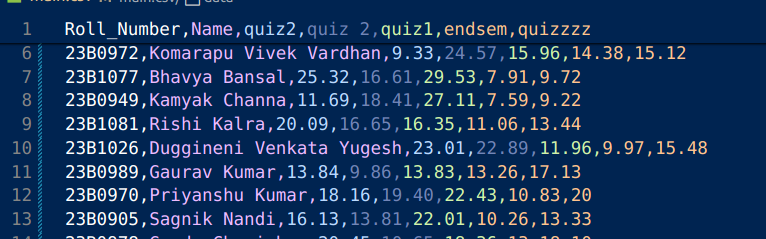
\includegraphics[width=0.6\textwidth]{Upload quizzz.png}
        \caption{main.csv after uploading quizzz.csv}
        \label{fig:upload}
    \end{figure}
    To remove an uploaded quiz, running
    \begin{lstlisting}
        bash submission.sh combine --drop quizzz.csv
    \end{lstlisting}
    Of course, this does not delete the copy of quizzzz.csv in the \texttt{WORKING\_DIRECTORY}, which will have to be done manually using rm.

    \section{Query}
    Finds the closest match either amongst Roll Numbers or the Names present in main.csv to the given query.\\
    If the query is a substring of a name or roll number, it is considered a match, and all strings of which it is a substring are returned.\\
    If it is not a substring of any name, the closest n matches are calculated using the Levenshtein distance between each word of the query and any word of the potential match.\\
    For instance "Aditya Neeraje" and "Neeraje Aditya" have a Levenshtein distance of 0, since "Aditya" and "Aditya" are the same, and "Neeraje" and "Neeraje" are the same.\\
    Using the \texttt{-n}/\texttt{--number} flag, you can specify the number of matches to return.\\
    Using the \texttt{-u}/\texttt{--uniq} flag, you can specify that only the roll number of the best match is to be returned, which other functions such as percentile and update make use of to get the closest roll number to the given query.\\
    \begin{lstlisting}
        bash submission.sh query Neraje -n 5
    \end{lstlisting}
    \begin{figure}[htbp]
        \centering
        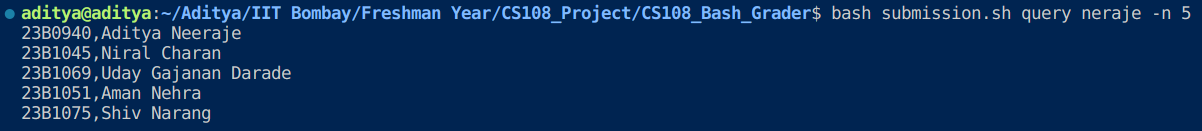
\includegraphics[width=0.8\textwidth]{Query Neraje.png}
        \caption{Querying for "Neraje" instead of Neeraje with 5 matches}
        \label{fig:query}
    \end{figure}
    An arbitrary number of queries can be passed at once to query, and the script will return the closest match to each query.\\

    \section{Percentile}
    Uses awk to calculate the percentile of a given student in each quiz. The spell-checking algorithm is run in the background.\\
    You can use the -r flag to specify to what number of decimal places to round the percentile.\\
    \begin{lstlisting}
        bash submission.sh percentile 23B0940 "Neeraje" 
                "Aditya Neeraje" "Neeraje Aditya"
    \end{lstlisting}
    \begin{figure}[htbp]
        \centering
        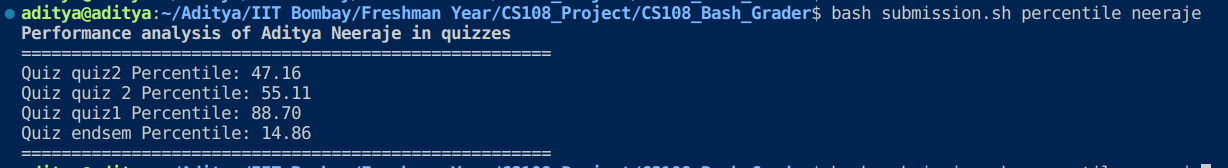
\includegraphics[width=0.8\textwidth]{Neeraje_percentile.png}
        \caption{Percentile of Neeraje}
        \label{fig:percentile}
    \end{figure}

    \section{Analyze}
    Uses percentile to get the percentile of the student in every quiz, then finds his average percentile. If his percentile in any quiz is somewhat or significantly lower than his average percentile. Analyze reports this. If the student has been consistent, average reports this.\\
    A percentile drop of between 10\% and 20\% below average is taken to be somewhat underwhelming, and a percentile drop of greater than 20\% is taken to be significant underperformance.

    \section{Total}
    Adds a total column to main.csv, with the columns to sum up determined by the user using the \texttt{-d}/\texttt{--drop} flag and the only flag, just like in combine.\\
    Assuming main.csv initially has all 4 quizzes, the following commands will have the following results:
    \begin{figure}[htbp]
        \centering
        \begin{subfigure}[b]{0.32\textwidth}
            \centering
            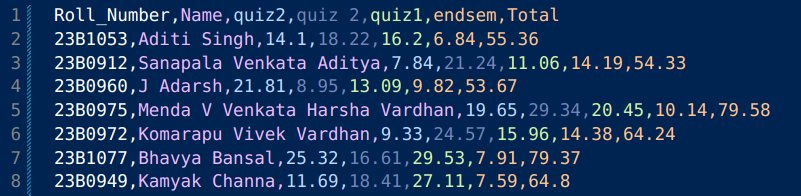
\includegraphics[width=\textwidth]{Total_All.png}
            \caption{total --force}
            \label{fig:sub1}
        \end{subfigure}
        \hfill
        \begin{subfigure}[b]{0.32\textwidth}
            \centering
            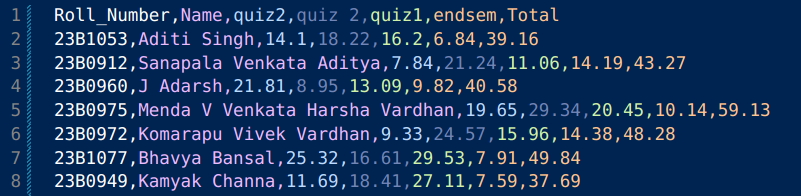
\includegraphics[width=\textwidth]{Total_drop_quiz1.png}
            \caption{total --force --drop quiz1.csv}
            \label{fig:sub2}
        \end{subfigure}
        \hfill
        \begin{subfigure}[b]{0.32\textwidth}
            \centering
            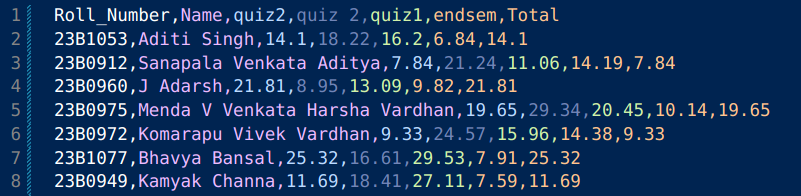
\includegraphics[width=\textwidth]{Total_only_quiz2.png}
            \caption{total quiz2.csv --force}
            \label{fig:sub3}
        \end{subfigure}
        \caption{main.csv after adding total}
        \label{fig:total}
    \end{figure}
    Note that without the force flag, if a total column is present in main.csv and it has valid numeric or "a" marks, the script will not evaluate the total column again.\\
    
    Note further that all commands, such as combine, upload, rescale and update keep track of which columns of main.csv were dropped earlier from total and drop them again while running total after the command is processed. For instance, running:
    \begin{lstlisting}
        bash submission.sh total --force --drop quiz1.csv
        bash submission.sh combine --drop quiz2.csv
    \end{lstlisting}
    \begin{figure}[htbp]
        \centering
        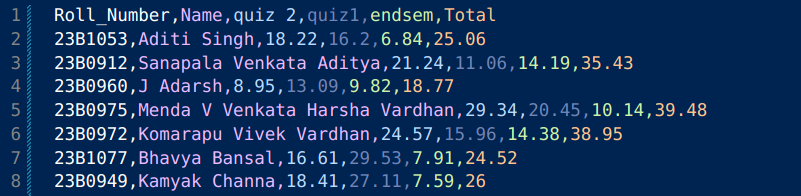
\includegraphics[width=0.4\textwidth]{Total_after_drop_and_combine.png}
        \caption{Even after combine, the Total column excludes quiz1.csv}
        \label{fig:total_after_combine}
    \end{figure}

    \begin{lstlisting}
        bash submission.sh total --force --drop quiz1.csv
        bash submission.sh rescale -w 1 2 1 1
    \end{lstlisting}
    \begin{figure}[htbp]
        \centering
        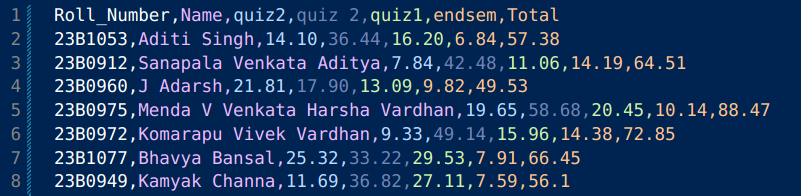
\includegraphics[width=0.4\textwidth]{Total_after_drop_and_rescale.png}
        \caption{Even after rescale, the Total column excludes quiz1.csv, but accounts for the doubling of quiz 2 marks}
        \label{fig:total_after_rescale}
    \end{figure}

    \section{Update}
    Accepts the quiz name, a query which is then searched against the list of roll numbers and student names, and the updated marks. Total is also updated keeping in mind quizzes which were previously dropped.
    \begin{figure}[htbp]
        \centering
        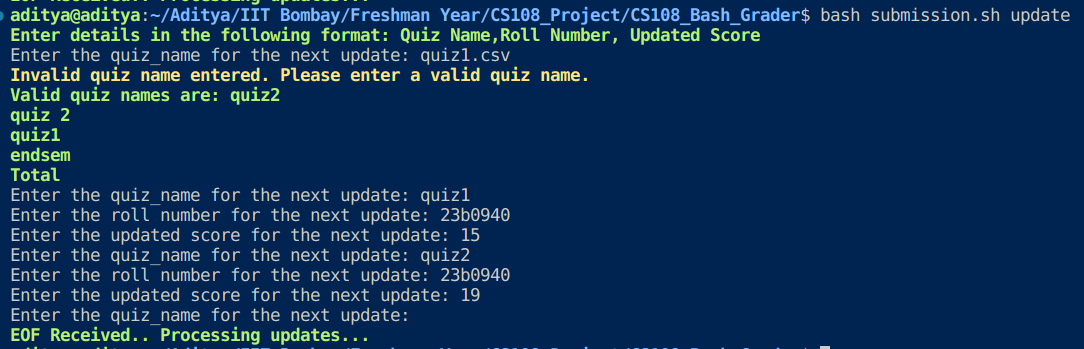
\includegraphics[width=0.8\textwidth]{Update command.png}
        \caption{Updating the marks of Neeraje}
        \label{fig:update}
    \end{figure}
    \begin{figure}[htbp]
        \centering
        
\includegraphics[width=0.8\textwidth]{Result of Update.png}
        \caption{main.csv after updating Neeraje's marks}
        \label{fig:update_result}
    \end{figure}

    Invalid details are handled as shown below:
    \begin{figure}[htbp]
        \centering
        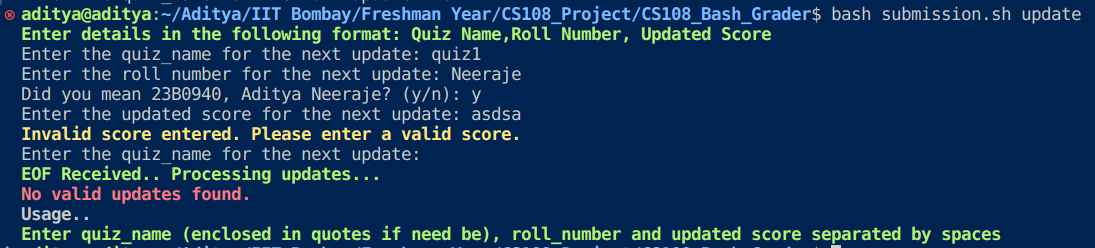
\includegraphics[width=0.8\textwidth]{Handling Invalid Details for Update.png}
        \caption{Invalid Update}
        \label{fig:invalid_update}
    \end{figure}

    Note that update after rescale is a case I have not handled, as only the field corresponding to the quiz name and student in main.csv is updated, hence the scaling factor is not automatically applied. For now, it is recommended to simply run rescale at the end, after all cribs.

    \section{git\_init}
    Initializes a git repository in the folder passed as an argument. A symlink called .my\_git is created that points to the given directory.\\
    I have implemented a for loop that allows for the directory to be created recursively even if some of the ancestors of the final directory mentioned do not exist. For example:
    \begin{lstlisting}
        bash submission.sh git_init ../Aditya/Neeraje/Hello/World
    \end{lstlisting}
    generates the entire sequence of directories: Aditya, Neeraje, Hello and World even if Aditya does not exist in the ../ directory.\\

    For now, let us run the command:
    \begin{lstlisting}
        bash submission.sh git_init Neeraje
    \end{lstlisting}
    This creates a directory Neeraje in \texttt{WORKING\_DIRECTORY} and creates a symlink to it.\\

    After at least one commit is made in the repository, calling git\_init again will prompt before shifting repositories. The .my\_git symlink now points to the new repository, which obtains all the commit history of the old repository.\\
    Due to a logical error in having reversed the order of the following two lines:
    \begin{lstlisting}
        grep -Ev "^$" "$WORKING_DIRECTORY/.my_git/.git_log" 
            > "$WORKING_DIRECTORY/$TEMPORARY_FILE" 2>/dev/null
        ln -s "$final_directory" "$WORKING_DIRECTORY/.my_git"
    \end{lstlisting}
    in the submission, the data stored in the .git\_log file is not copied while reinitializing the git repository. That bug has since been corrected and pushed to my GitHub repository\cite{url:github}.\\
    Also, due to another logical error, if the git repository had been initialized but the .git\_log file was empty due to a lack of commits, running git\_init again would not shift the git repository. This was because the deletion of the symlink occurs inside an if statement that requires the non-emptiness of the .git\_log file to be entered. This error has been resolved as well.\\

    \section{git\_commit}
    \begin{lstlisting}
        bash submission.sh git_commit -m "First commit - All Files"
    \end{lstlisting}

    Due to a logical error, git\_commit does not copy and store main.csv. That has been modified by the use of the following lines in the latest version:
    \begin{lstlisting}
        selected_quizzes+=("$WORKING_DIRECTORY/main.csv")
        for quiz in "${quizzes[@]}"; do
            if [[ -f "$quiz" ]]; then
                selected_quizzes+=("$quiz")
            fi
        done    
    \end{lstlisting}
    This ensures that main.csv is always included in the list of files to be committed.\\
    \begin{figure}[htbp]
        \centering
        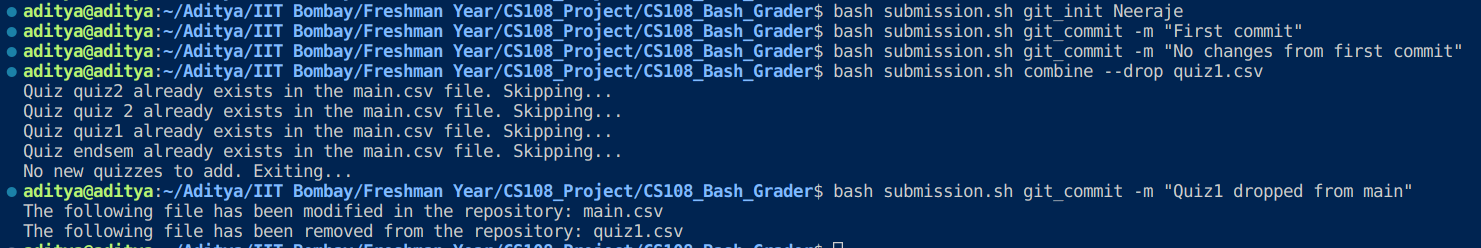
\includegraphics[width=0.8\textwidth]{Git Commit history.png}
        \caption{Some commands to generate commits}
        \label{fig:first_commit}
    \end{figure}
    \begin{figure}[htbp]
        \centering
        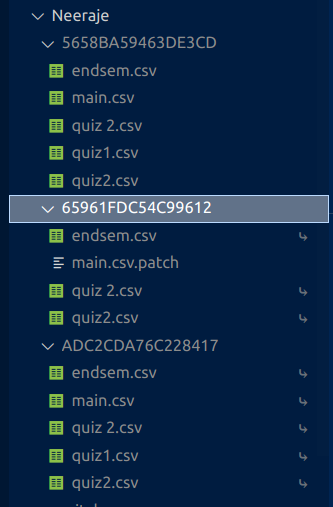
\includegraphics[width=0.4\textwidth]{How Files are Stored.png}
        \caption{How the files are stored}
        \label{fig:second_commit}
    \end{figure}
    As you can see, the first commit stores all the files as csv files. The second commit, which has no changes relative to the first, stores all files as symlinks. The third commit, where quiz1.csv is dropped, stores all files except main.csv as symlinks. main.csv is stored as a patch file.\\
    \begin{figure}[htbp]
        \centering
        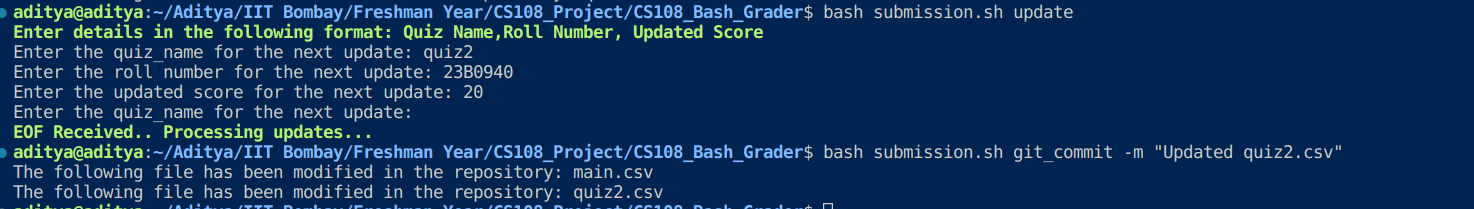
\includegraphics[width=0.4\textwidth]{Git Commit after an update.png}
        \caption{Git commit after an update, shows that main.csv and quiz2.csv have been modified}
        \label{fig:third_commit}
    \end{figure}
    After this update, quiz2.csv is also stored as a patch file.

    \begin{figure}[htbp]
        \centering
        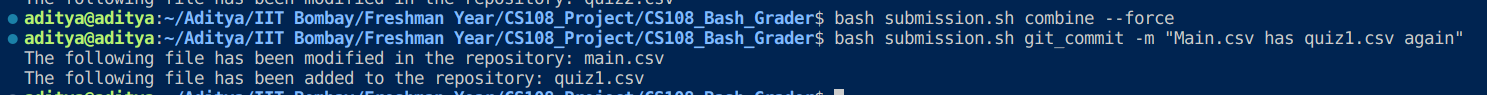
\includegraphics[width=0.8\textwidth]{Git commit after maincsv has quiz1 again.png}
        \caption{Git commit after force combining main.csv, shows that quiz1.csv has been added again. quiz1.csv is still a symlink in the remote.}
        \label{fig:fourth_commit}
    \end{figure}

    git\_commit --amend with an optional message allows you to amend the last commit. The last commit data is still stored, but it no longer shows up in git\_log.\\
    \begin{lstlisting}
        bash submission.sh git_commit --amend -m "Amended prev commit"
        bash submission.sh git_commit --amend
    \end{lstlisting}
    \begin{figure}[htbp]
        \centering
        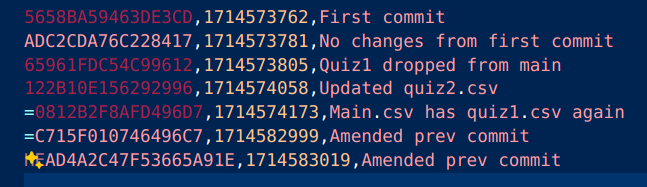
\includegraphics[width=0.8\textwidth]{commit_amend.png}
        \caption{.git\_log after amending the last commit}
        \label{fig:amend_commit}
    \end{figure}

    If no commit message is specified, the script gets a commit message from the internet from https://whatthecommit.com/. I am not personally responsible for the language of these prompts. Using the up arrow, w or W, the user can choose to use these commits for his commit message. With a one in five probability, a certain Easter egg appears.\\

    \section{git\_add and git\_remove}
    These modify the .my\_gitignore file to specify certain files to always copy or to always exclude during git\_commit. .my\_gitignore can handle the same regex expressions that can be handled by bash, as well as the ! command before the regex to indicate not to ignore the file ever. my\_gitignore is parsed from top to bottom, so ignoring a file once and then unignoring it will cause it to not be ignored, and vice versa.\\
    To view which files are being tracked:
    \begin{lstlisting}
        bash submission.sh git_remove quiz1.csv "quiz 2.csv"
        bash submission.sh git_status
    \end{lstlisting}
    \begin{figure}[htbp]
        \centering
        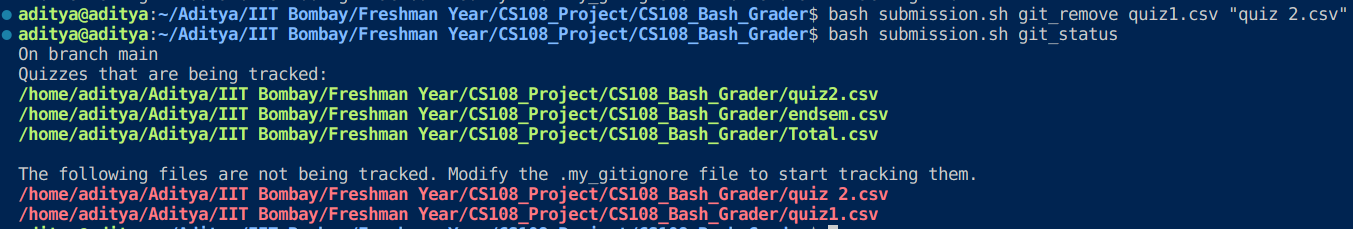
\includegraphics[width=0.8\textwidth]{git_status_some_quizzes_removed.png}
        \caption{git\_status with quiz1 and quiz 2 not tracked}
        \label{fig:git_status}
    \end{figure}
    To add all csv files present in the \texttt{WORKING\_DIRECTORY}:
    \begin{lstlisting}
        bash submission.sh git_add .
        (or) bash submission.sh git_add *
    \end{lstlisting}
    Equivalent commands work for git\_remove, or you can equivalently pass the -r flag to git\_add to specify removal instead of addition.\\
    \begin{figure}[htbp]
        \centering
        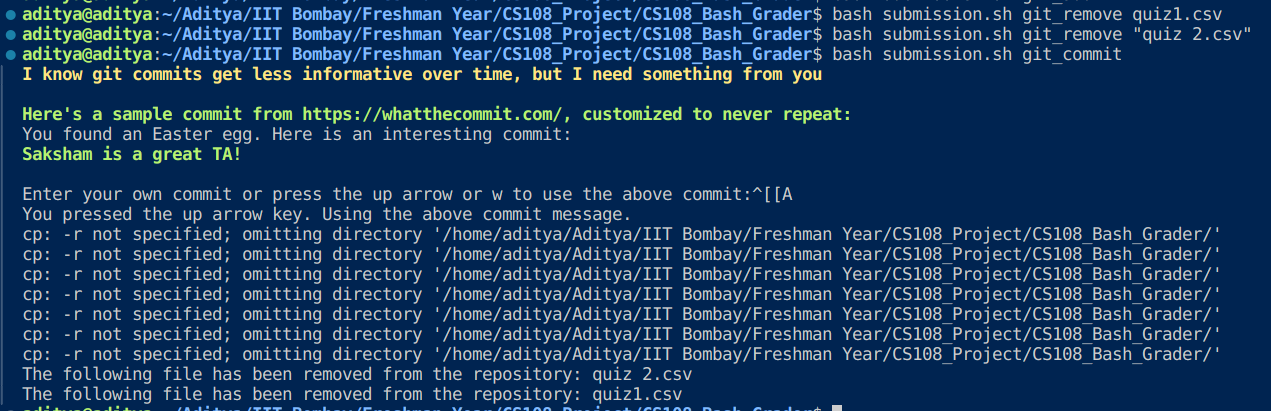
\includegraphics[width=0.8\textwidth]{committing after git remove.png}
        \caption{Committing after git\_remove is called. Note that quiz1.csv and quiz 2.csv are not tracked.}
        \label{fig:git_status_all}
    \end{figure}
    The cp errors are expected, since parse\_gitignore works by calling:
    \begin{lstlisting}
        selected_quizzes=("${selected_quizzes[@]/$quiz}")        
    \end{lstlisting}
    which replaces the instance of \$quiz in the array with a blank space. These error messages can safely be suppressed, since they try to make cp copy the \texttt{WORKING\_DIRECTORY}, which fails in the absence of the recursive flag. 

    \section{git\_checkout}
    This command checks out the commit whose hash is closest to the query hash passed as an argument. If no existing hash is within a Levenshtein distance of 5 to the query hash, it reports the same.\\
    The query must at least be of length 4.\\
    git\_checkout also checks whether the local directory is the same as either the commit you are checking out or the latest two commits in .git\_log. If not, it prompts the user to save the local repository as a commit.\\
    The reason for checking out the latest two commits was because otherwise, if you check out a commit A different from the latest commit B, and you call git\_checkout main, the script prompts you to store the local directory as commit C, which is chronologically after commit B. If you git\_checkout main again, commit C is the latest commit, but then commit B and commit C are different, so B is stored as a new commit D, and so on, creating an infinite loop where git\_checkout main never is actually at the tip of main unless the force flag is used.\\

    If there have been changes in the local repository, git\_checkout prompts for the new commit to be saved before checking out the commit.\\
    It also tells the user what files have changed, been added or deleted.\\
    \begin{figure}[htbp]
        \centering
        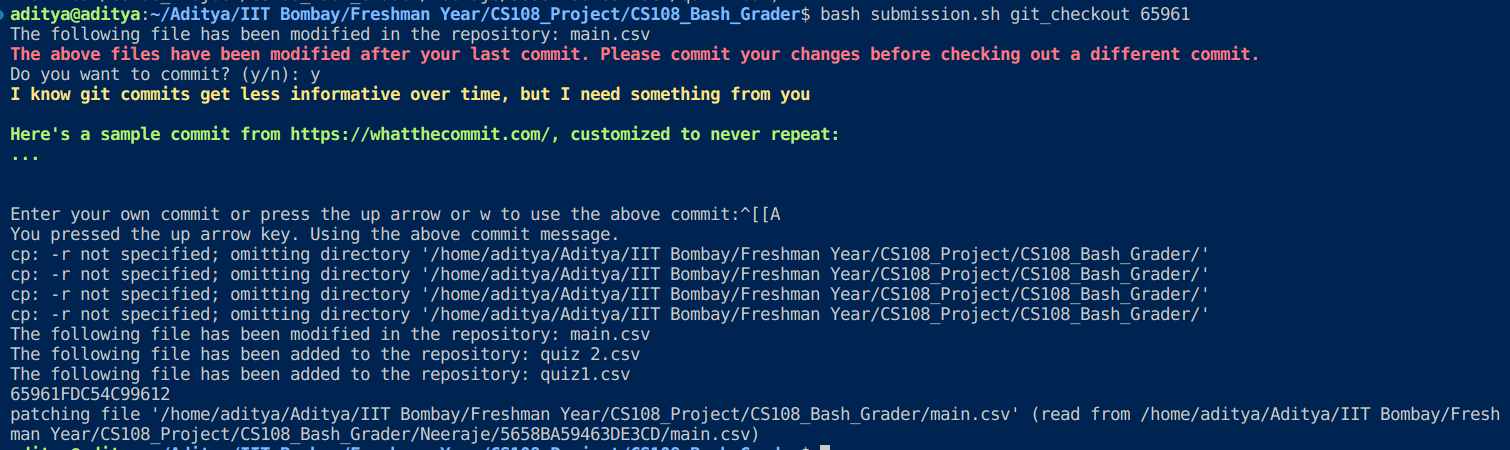
\includegraphics[width=0.8\textwidth]{git_checkout_65961_from_122B.png}
        \caption{git\_checkout of commit 6596 when at commit 122B prompts for the local repository to be stored as a new commit, as the local repository is not equivalent to either of the two most recent commits. The addition of quiz 2.csv and quiz1.csv is because the latest commit in .git\_log was committed after git\_remove was called, and hence did not have quiz1 or quiz 2.}
        \label{fig:git_checkout}
    \end{figure}
    \begin{figure}[htbp]
        \centering
        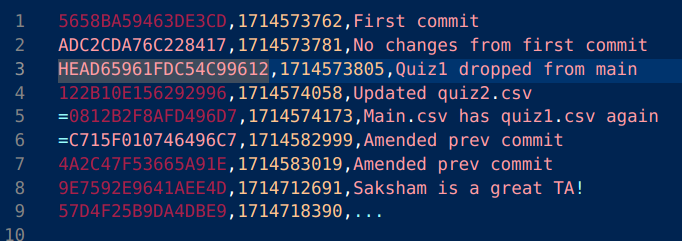
\includegraphics[width=0.8\textwidth]{git log file after checkout.png}
        \caption{git\_log after git\_checkout. Note that the position of HEAD has changed. Also, the local repository is stored as the new commit with hash 57D4.}
        \label{fig:git_checkout_same}
    \end{figure}

    \section{Grade}
    If main.csv already has a total column, grade prompts the user on whether to use the same total column to display a scatterplot of the sorted marks, as well as recommended grade cutoffs for AP, AA, AB, BB, BC, DD (assuming all people lower than DD are FRs).\\
    First, a bell-curve type distribution is created by taking the mean, mean + 30/weightage, mean + 20/weightage, etc. where weightage is the 100/maximum\_marks. Then, on the sorted list of totals, the biggest jump in the vicinity of these cutoffs is taken to be the final cutoff.\\
    By using different values for the variable WIDTH, I figured out that the best looking graphs came when I searched for the biggest jump in an interval of width $\frac{bucket\_width}{2}$ around the cutoff, where bucket\_width is the distance between the current cutoff and the immediately higher cutoff (with the highest cutoff being the number of students).\\
    \begin{lstlisting}
        bash submission.sh grade
    \end{lstlisting}
    \begin{figure}[htbp]
        \centering
        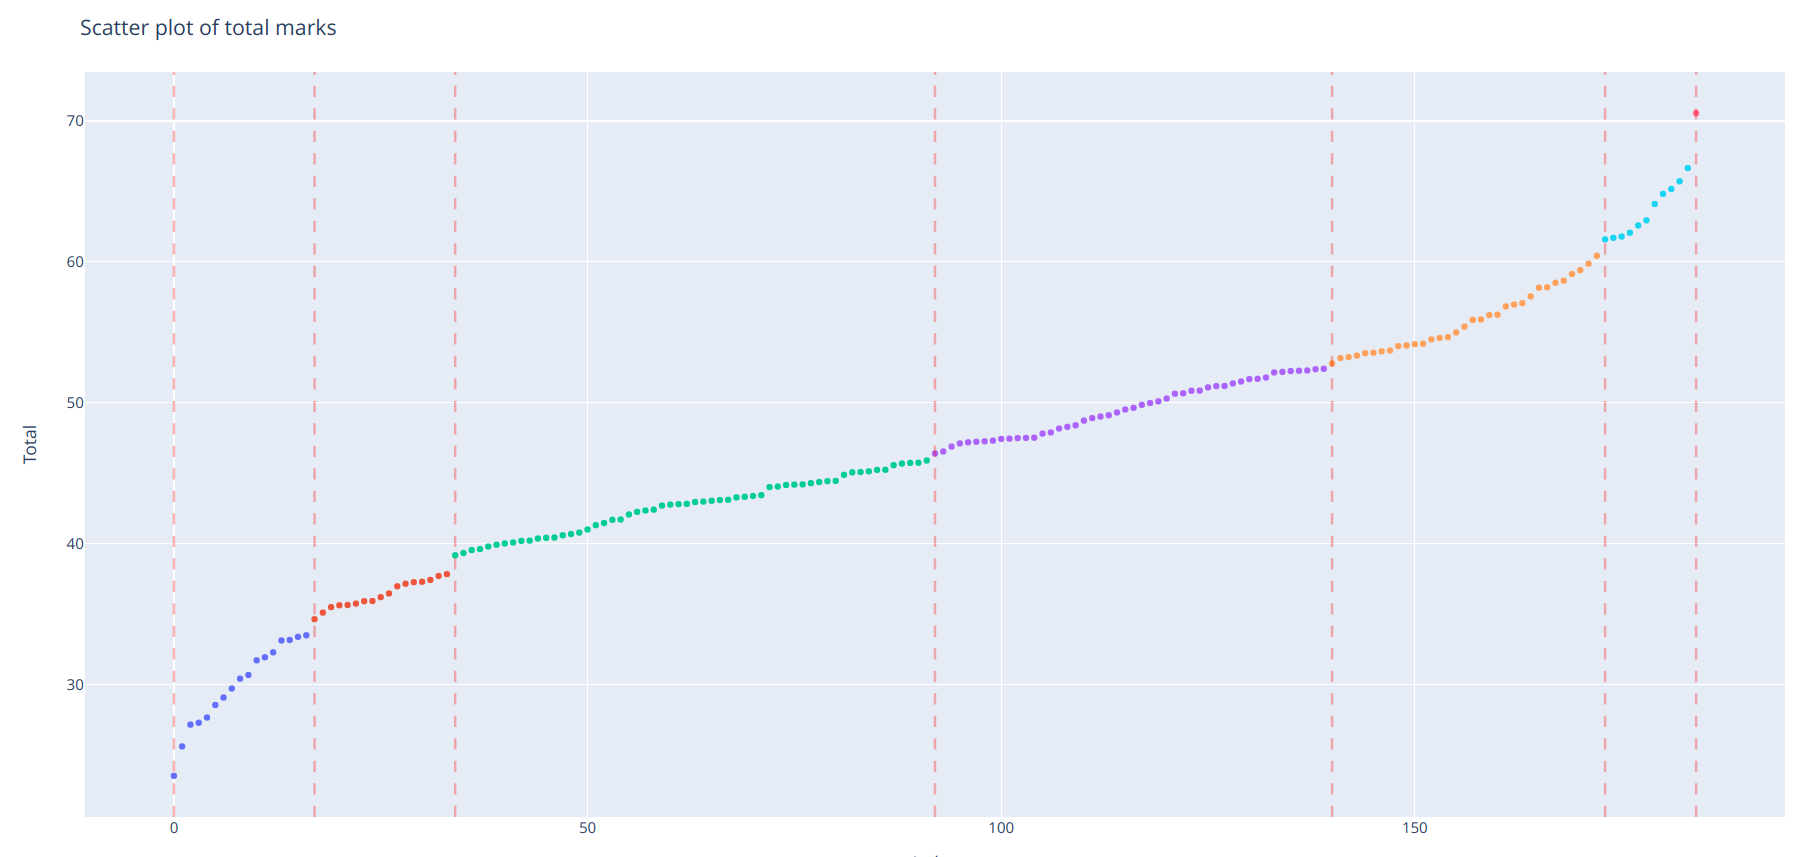
\includegraphics[width=0.8\textwidth]{Grade.png}
        \caption{Grade command}
        \label{fig:grade}
    \end{figure}

    \section{grade\_manual}
    I even have a grade\_manual command that allows the user to specify the cutoffs for each grade.\\
    On a desktop with wayland enabled, matplotlib displays the graph, and the cutoff vertical line moves along with the user's cursor and changes color according to the grade whose cutoff it is. The cutoff line does not move more right than the previous cutoff, however, reflecting the fact that the cutoffs must always be in decreasing order.\\
    As with grade, the user is prompted on whether to use a pre-existing Total column, if any.\\
    Both grade and grade\_manual generate a main.html file which stores the students' data and grades in tabular form.\\

    \section{report\_card}
    Generates a report card for the student whose name or roll number is queried, using a latex template present in the Report\_Cards\_Template folder.\\
    \begin{figure}[htbp]
        \centering
        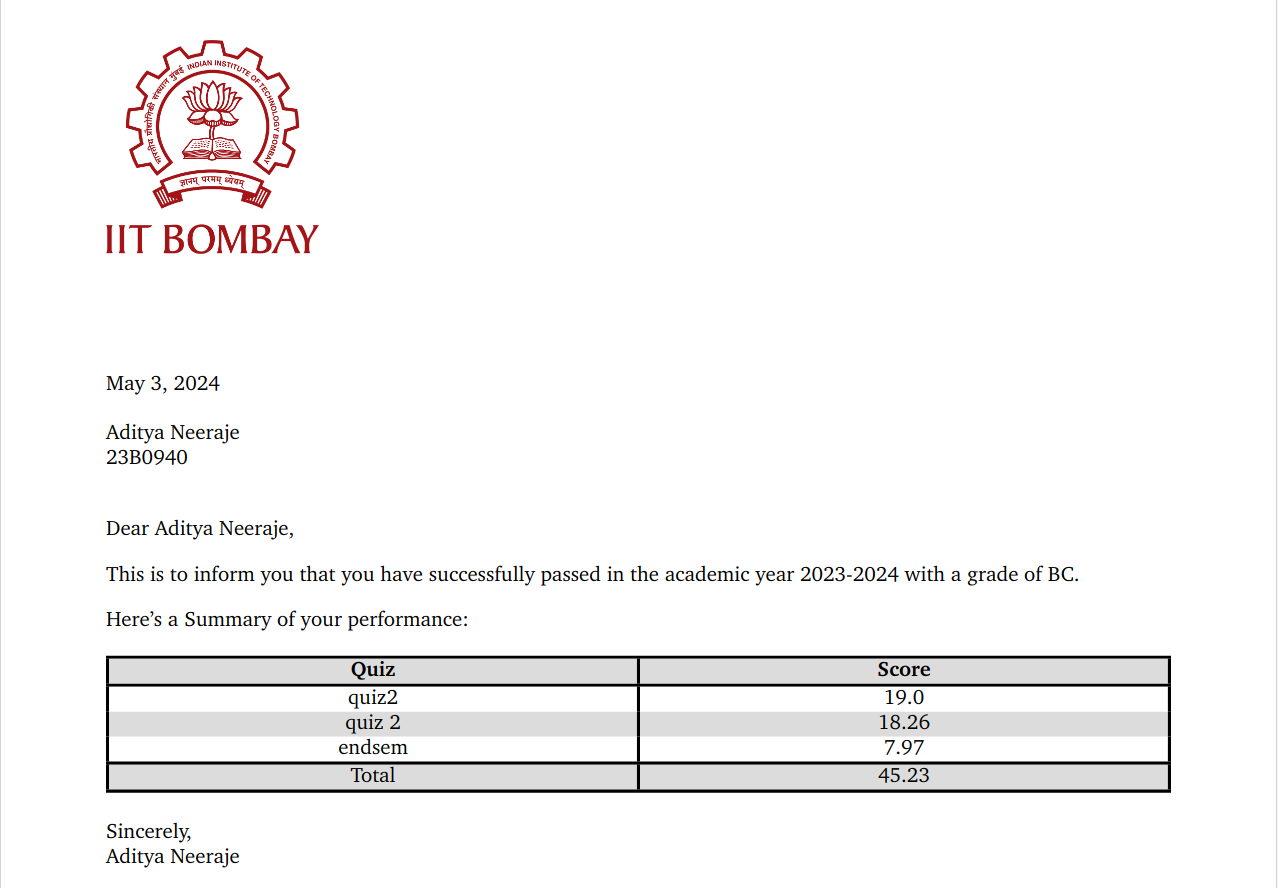
\includegraphics[width=0.8\textwidth]{report_card.png}
        \caption{Report Card for Neeraje}
        \label{fig:report_card}
    \end{figure}
    If no argument is specified, report cards are generated for every student in main.csv. This takes up significant time, so it is not recommended to run this during the viva session unless at the end.

    \section{git\_log}
    If you are in detached HEAD state, git\_log reports that and exits. If not, it prints the hash, commit time and commit message of all the commits until the HEAD is reached. Commits which have been "forgotten" due to being amended later on are not shown.
    Using the \texttt{--oneline} flag, only the commit hash and commit message can be displayed, each commit taking up one line.
    
    \section{display\_boxplot and display\_stripplot}
    Generic plotly express boxplot and stripplot of the quizzes. If rescale is specified, the plots are all rescaled such that their maximums are at the value passed as an argument to rescale (default is 100 if the \texttt{-r}\texttt{--rescale} flag is passed).\\
    If a rescale value of 0 is passed, it is ignored. If a non-numeric or negative rescale value is passed, the graph is rescaled to 100.

    \begin{lstlisting}
        bash submission.sh boxplot --rescale 100
    \end{lstlisting}
    \begin{figure}[htbp]
        \centering
        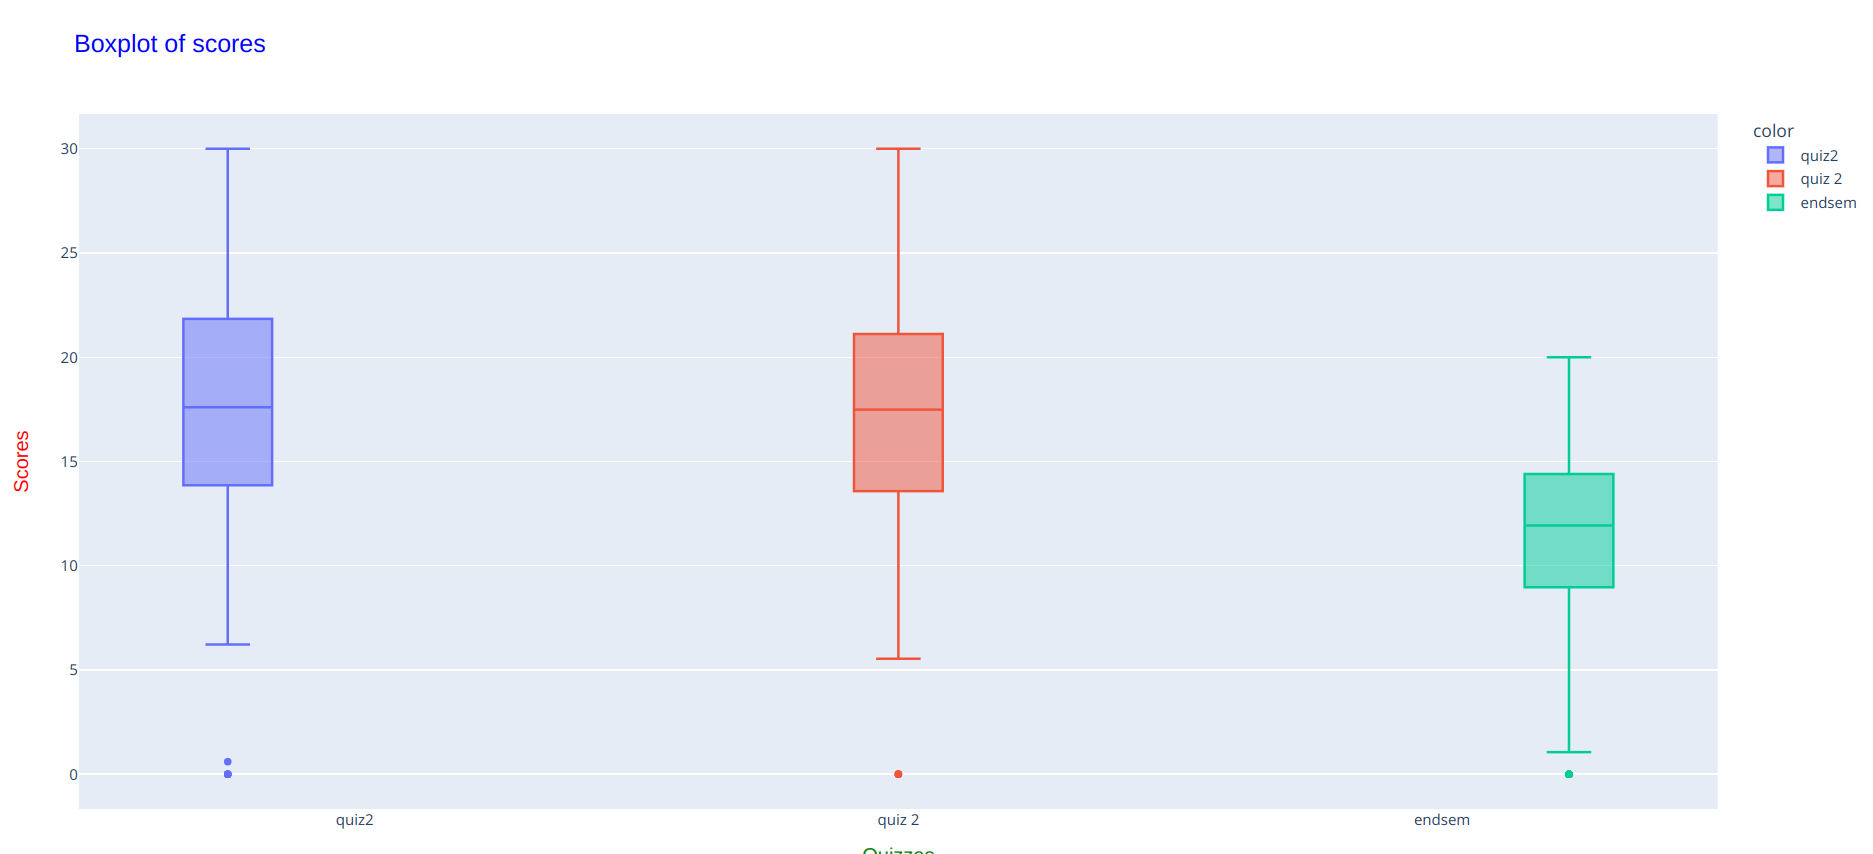
\includegraphics[width=0.8\textwidth]{boxplot_of_scores.png}
        \caption{Boxplot of the quizzes}
        \label{fig:boxplot}
    \end{figure}
    \printbibliography
\end{document}

